\documentclass{article}
\usepackage{amsmath}
\usepackage{color}
\usepackage{tikz}
\usetikzlibrary{arrows.meta}

\begin{document}

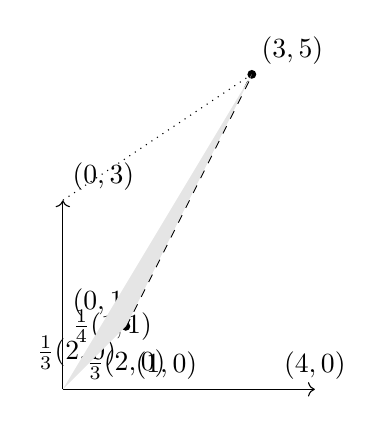
\begin{tikzpicture}[scale=0.8]
    % Define coordinates
    \coordinate (O) at (0,0);
    \coordinate (A) at (4,0);
    \coordinate (B) at (0,3);
    \coordinate (C) at (1,0);
    \coordinate (D) at (0,1);
    \coordinate (E) at (3,5);
    \coordinate (F) at (1,1);
    
    % Draw lines and arrows
    \draw[->] (O) -- (A); % x-axis
    \draw[->] (O) -- (B); % y-axis
    \draw[thick, dashed] (F) -- (E); % beta^can
    \draw[dotted] (E) -- (0,3); % beta^res
    \fill (F) circle[radius=2pt];
    \fill (E) circle[radius=2pt];
    
    % Annotate points
    \node at (E) [above right] {$(3,5)$};
    \node at (F) [below left] {$\frac{1}{3}(2,0)$};
    \node at (0,1) [above right] {$(0,1)$};
    \node at (0,3) [above right] {$(0,3)$};
    \node at (1,0) [above] {$\frac{1}{3}(2,0)$};
    \node at (0,1) [right] {$\frac{1}{4}(1,1)$};
    \node at (1,0) [above right] {$(1,0)$};
    \node at (4,0) [above] {$(4,0)$};

    % Fill region
    \fill[gray!20] (O) -- (F) -- (E) -- cycle;
\end{tikzpicture}

\textbf{For } \$W = \Sym^3 V \oplus \Sym^2 V \otimes \det V\$ \textbf{, the Newton polygon } \$\Lambda^u\$ \textbf{ at } \$u \in \bf{P}^1\$ \textbf{ with the vanishing orders } \$r_1 = 2\$ \textbf{ and } \$r_2 = 0\$ \textbf{. The short normal vectors (dashed) represent } \$\beta^{\rm can}\$ \textbf{ and the longer ones (dotted) represent } \$\beta^{\rm res}\$.

\end{document}